\documentclass[11pt]{article}
\usepackage[english]{babel}
\usepackage[utf8]{inputenc}
\usepackage{fancyhdr}
\usepackage{graphicx}

\def\Name{Ran Liao}
\def\Topic{Use-Case Diagram}

\title{\textbf{\Topic}}
\author{\Name}
\markboth{Notes on \Topic\ }{Notes on \Topic\ }
\date{\today}
 
\pagestyle{fancy}
\fancyhf{}
\rhead{\date{\today} }
\lhead{Notes on \Topic\ }
\rfoot{\thepage}

\textheight=9in
%\textwidth=6.5in
\topmargin=-.75in
%\oddsidemargin=0in
%\evensidemargin=0in
 
\begin{document}
\maketitle
\noindent\makebox[\linewidth]{\rule[8pt]{5in}{0.5pt}}


\section*{Overview}
A use case is a model of the interaction between external users of a software product (actors) and the software product itself. A use-case diagram is a set of use cases

\section*{Actor}

An actor is a member of the world outside the software product. A user of the system can play more than one role. Conversely, one actor can be a participant in multiple use cases. And an actor need not be a human being. Generalization of actors is supported and denoted by an open triangle points toward the more general case.

\begin{figure}[h]
	\centering
	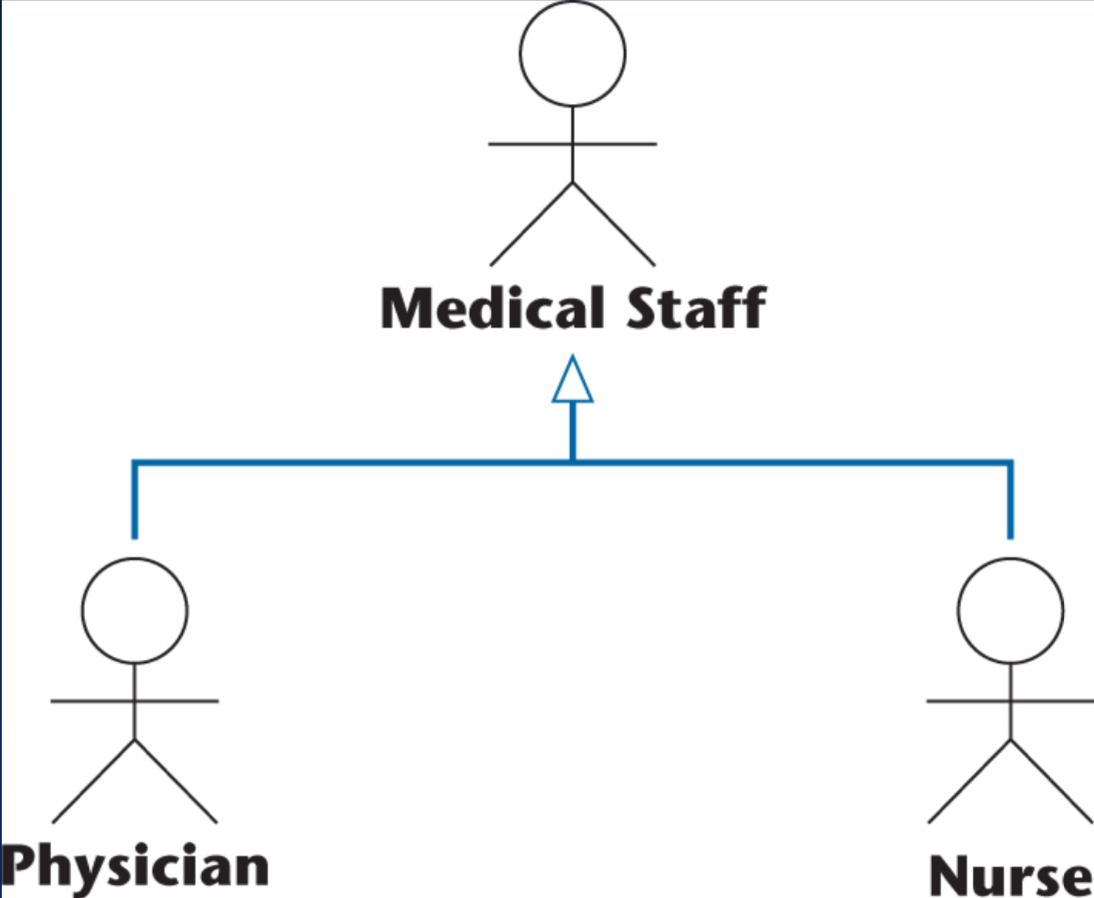
\includegraphics[width=0.4\linewidth]{images/GeneralizationActor.png}
	\caption{Generalization of Actors}
	\label{fig:GeneralizationActor}
\end{figure}

\section*{Stereotypes}
 
A stereotype in UML is a way of extending UML and the names of stereotypes appear between guillemets.

\begin{itemize}
	\item \textbf{«include»}
	
	In the «include» relationship, one use case is part of another use case.
	
	\begin{figure}[h]
		\centering
		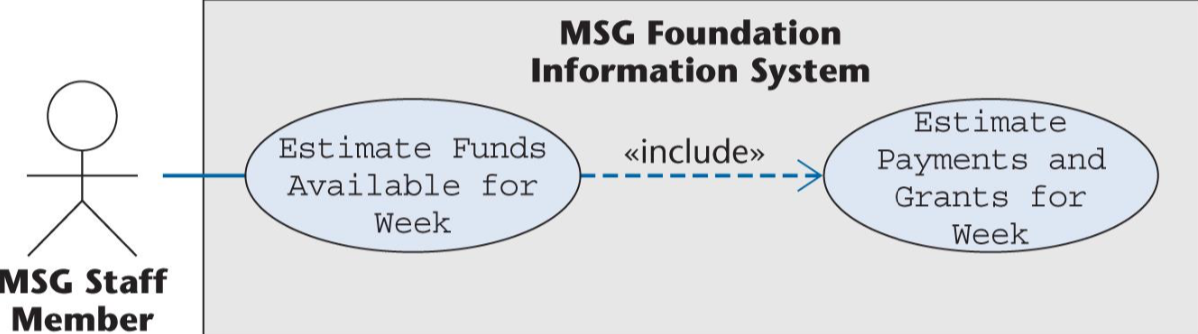
\includegraphics[width=0.8\linewidth]{images/Include.png}
		\caption{Include Stereotypes}
		\label{fig:Include}
	\end{figure}

	\item \textbf{«extend»}
	
	In the «include» relationship, one use case is a variation of the standard use case.
	
	\begin{figure}[h]
		\centering
		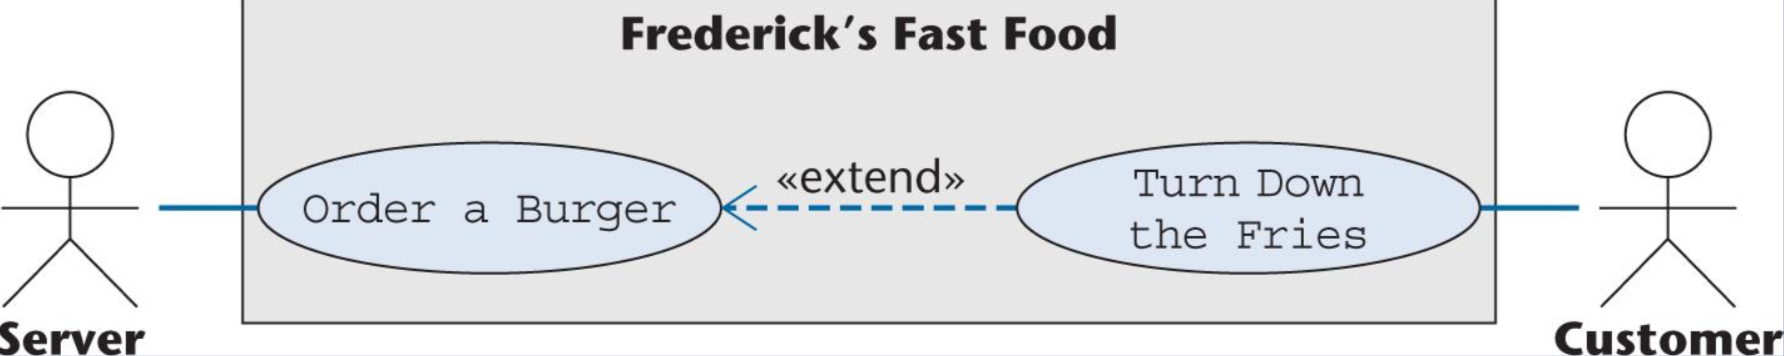
\includegraphics[width=0.8\linewidth]{images/Extend.png}
		\caption{Extend Stereotypes}
		\label{fig:Extend}
	\end{figure}
\end{itemize}



\end{document}